\chapter{Nomenclature de la métrologie}

La métrologie traite de la relation entre mesure et instruments de mesure, qui sont deux choses fort différentes. Le concept de mesure et le concept d'instrument englobent un certain nombre de notions fondamentales, décrites ci-après.

\section{Nomenclature propre à la mesure}

\subsection{Le mesurage}

C'est \textbf{l'opération} consistant à mesurer une des caractéristiques d'un objet physique, et que la plupart d'entre nous appellent, de manière inexacte, la mesure.

\subsection{Le mesurande}

C'est l'observable (la grandeur physique) soumise au mesurage.

\subsection{La mesure}

La mesure est le \textbf{résultat numérique} de l'opération de mesurage appliquée au mesurande.

\subsection{L'incertitude sur la mesure}

C'est l'intervalle numérique autour de la valeur mesurée dans lequel on \textit{estime} que se trouve la vraie valeur de l'observable, avec une \textit{certaine} probabilité.\footnote{voir la partie du cours de métrologie concernant l'analyse des données expérimentales}

\subsection{Traçabilité des mesurages}

\begin{wrapfigure}[18]{r}[0pt]{10cm}
    \centering
    \vspace{-5mm}
    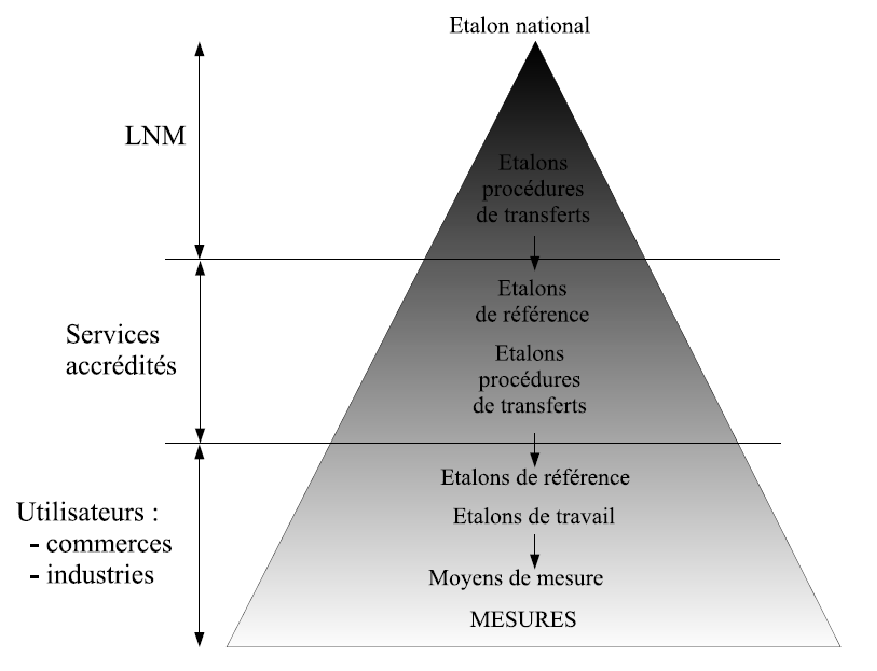
\includegraphics[width=10cm]{assets/figures/pyramideTracabilite.pdf}
    \caption{Pyramide de la traçabilité}
    \label{fig:pyr}
\end{wrapfigure}
La traçabilité est la propriété du résultat d'un mesurage tel qu'il puisse être relié à des références déterminées, généralement des étalons nationaux ou internationaux, par l'intermédiaire d'une chaîne ininterrompue de comparaisons ayant toutes des incertitudes déterminées. Son organisation est pyramidale (figure \ref{fig:pyr}), c'est-à-dire de la référence nationale (et/ou internationale) vers l'utilisateur. Les Laboratoires Nationaux de métrologie (LNM) détiennent les références nationales et les diffusent vers l'utilisateur. En Suisse, il s'agit du METAS - \texttt{http://www.metas.ch}

\section{Nomenclature propre aux instruments de mesure}

 (Ce paragraphe est fortement inspiré de la page \texttt{wikipedia} dédiée à la métrologie). Les principales caractéristiques des instruments de mesure (ou propriétés métrologiques des dispositifs de mesure) sont définies dans le cadre du Vocabulaire international de métrologie (VIM). Nous les décrivons ci-dessous.

\subsection{Étalonnage ou calibration}

L'étalonnage d'un instrument de mesure consiste à mesurer un mesurande de valeur numérique parfaitement connue (étalon ou calibre) et d'ajuster le système de mesurage propre à l'instrument de manière à ce que la valeur donnée corresponde à la valeur du mesurande étalon.

En règle générale, tout instrument de mesure est sujet à une dérive de sa réponse - en raison du vieillissement des ses composants internes (usure mécanique p. ex.) -  et nécessite un étalonnage périodique.

\begin{wraptable}[22]{r}[0pt]{4.5cm}
    \vspace{-1.5cm}
    \caption{Calibration d'un thermocouple, un exemple pratique.}
    \begin{center}
        \begin{tabular}{c|c}
            $T_e$ [$^\circ$C] & $U_e$ [V] \\
            10                & 5.43      \\
            11                & 6.21      \\
            12                & 7.19      \\
            13                & 8.16      \\
            14                & 9.11      \\
            15                & 10.31     \\
            16                & 11.35     \\
            17                & 12.55     \\
            18                & 13.73     \\
            19                & 15.38     \\
            20                & 16.67     \\
            21                & 18.36     \\
            22                & 20.29     \\
            23                & 22.03     \\
            24                & 24.13     \\
            25                & 26.33     \\
            26                & 28.77     \\
            27                & 30.73     \\
            28                & 33.27     \\
            29                & 35.89     \\
            30                & 38.09
        \end{tabular}
    \end{center}
    \label{tab:tc}
\end{wraptable}

\begin{flushleft}
    \underline{\textbf{Dans le cas d'un système simple}}
\end{flushleft}
Par exemple une balance ou un pied à coulisse. On peut se contenter d'un étalonnage dit à \textbf{un point}: on pèse par exemple une masse étalon, et on corrige la position de l'aiguille de la balance pour que celle-ci indique la valeur correcte. Cependant, cela ne suffit pas toujours. L'instrument peut en effet présenter:
\paragraph{une dérive systématique:} il indique systématiquement une valeur supérieure ou inférieure d'une \textbf{quantité fixe}; dans ce cas, la mesure est égale à la mesure vraie $m_v$ plus une quantité fixe $m_0$, $m=m_v+m_0$; si c'est le cas, la calibration permet de s'affranchir immédiatement de cette erreur systématique;
\paragraph{une dérive de sensibilité:} il indique systématiquement une valeur supérieure ou inférieure d'une \textbf{proportion donnée}; dans ce cas, l'erreur $m_0$ est proportionnelle à $m_v$, $m_0=\alpha\,m_v$, $m=m_v\,(1+\alpha)$; il convient alors de réaliser un étalonnage sur toute l'étendue de mesurage de l'instrument, de manière à vérifier qu’ $\alpha$ est bien constante.

\begin{flushleft}
    \underline{\textbf{Dans le cas d'instruments de mesure complexes}}
\end{flushleft}
On préfère généralement établir une \textbf{courbe de calibration} (figure \ref{fig:tc}), en suivant la procédure ci-dessous:
\paragraph{1/ Sélection des étalons.} On commence par sélectionner un grand nombre de mesurandes étalons de valeurs numériques $E$ comprises dans l'étendue de mesurage de l'instrument, distribuées de la manière la plus régulière possible. Considérons le cas pratique de l'étalonnage d'un thermomètre à thermocouple\footnote{il s'agit de deux fils conducteurs métalliques de composition différente, soudée; on peut observer alors entre les deux fils une différence de potentiel électrique qui va croitre avec la température de la soudure; il est évident qu'un thermomètre à thermocouple doit être calibré, c.-à-d. que l'on aura besoin de connaitre la courbe tension-température afin de l'utiliser.}: on plongera le thermocouple dans un même liquide à diverses températures (parfaitement connues) et ces températures constitueront notre base d'étalons, comme par exemple les températures données en table~\ref{tab:tc}, que nous allons utiliser pour notre exemple pratique;
\begin{wraptable}[11]{r}[0pt]{4cm}
    \vspace{-3mm}
    \caption{Écart-type entre modèle et mesures, pour un degré croissant du modèle polynomial.}
    \begin{center}
        \begin{tabular}{c|c}
            degré & $\sigma$ [$^\circ$C] \\
            1     & 1.010                \\
            2     & 0.288                \\
            3     & 0.060                \\
            4     & 0.054                \\
            5     & 0.054
        \end{tabular}
    \end{center}
    \label{tab:tc2}
\end{wraptable}
\paragraph{2/ Mesurage des étalons.} On effectue un mesurage de chacune des valeurs étalon\footnote{éventuellement, si on constate que l'affichage du voltmètre n'est pas très stable, on effectuera plusieurs mesures à chaque valeur de la tension, et on considérera la moyenne.}, et on note $M(E)$ la valeur donnée par l'appareil - qui n'est pas forcément dans les mêmes unités que $E$; pour le thermocouple $M(E)$ sera la tension mesurée entre les deux fils pour une certaine température du liquide; on aura donc 21 valeurs de la tension $U_e=M(T_e)$ - la mesure est en volts, mais l'étalon est en $^\circ$C; voir table~\ref{tab:tc} pour les valeurs de $U_e$ mesurées avec notre thermocouple;

\paragraph{3/ Les données.} Les couples (étalon $E$, mesure $M(E)$) sont chargés dans un logiciel de traitement de données (MATLAB, par exemple); mais attention~! à présent, on inverse le problème: en effet, par exemple dans le cas du thermocouple, ce que l'on désire, c'est une courbe de calibration, c'est-à-dire une fonction mathématique qui permette, à partir de la donnée de la tension électrique $U$ mesurée, de donner la valeur correspondante de la température de la soudure, au plus juste; par conséquent, les mesures $M(E)$ (ici $U(T)$) constituent la variable d'\textbf{entrée}, et les valeurs étalons $E$ (ici $T$) la variable de \textbf{sortie};

\paragraph{4/ Recherche de la courbe de calibration.} On ajuste un modèle mathématique (par exemple ci-dessous un polynôme, ou alors une exponentielle, un cosinus, ou une combinaison de fonctions de base, etc.) $$\mathcal{C}(M)=a_0+a_1M+a_2M^2+a_3M^3+\dots$$ sur les couples ($M(E)$, $E$). L'ajustement consiste à trouver la valeur des paramètres $a_0, a_1, a_2,\dots$ qui permet d'obtenir l'écart minimal entre mesures et modèle. Le modèle optimal constituera notre courbe de calibration $\mathcal{C}(M)$.

Par exemple, pour le thermocouple, si on calcule l'écart-type moyen entre les données et un modèle polynomial, on trouve que le degré 4 est optimal - car au-delà, il n'y a pratiquement aucun gain de précision (voir table~\ref{tab:tc2}), et la courbe de calibration est donnée par:
\begin{equation*}
    \mathcal{C}_T(U)=2.439+1.621\,U-4.522\,10^{-2}\,U^2+7.221\,10^{-4}\,U^3-4.039\,10^{-6}\,U^4\ \ \text{[$^\circ$C]}
\end{equation*}

\begin{wrapfigure}[15]{r}[0pt]{7cm}
    \vspace{-0mm}
    \centering
    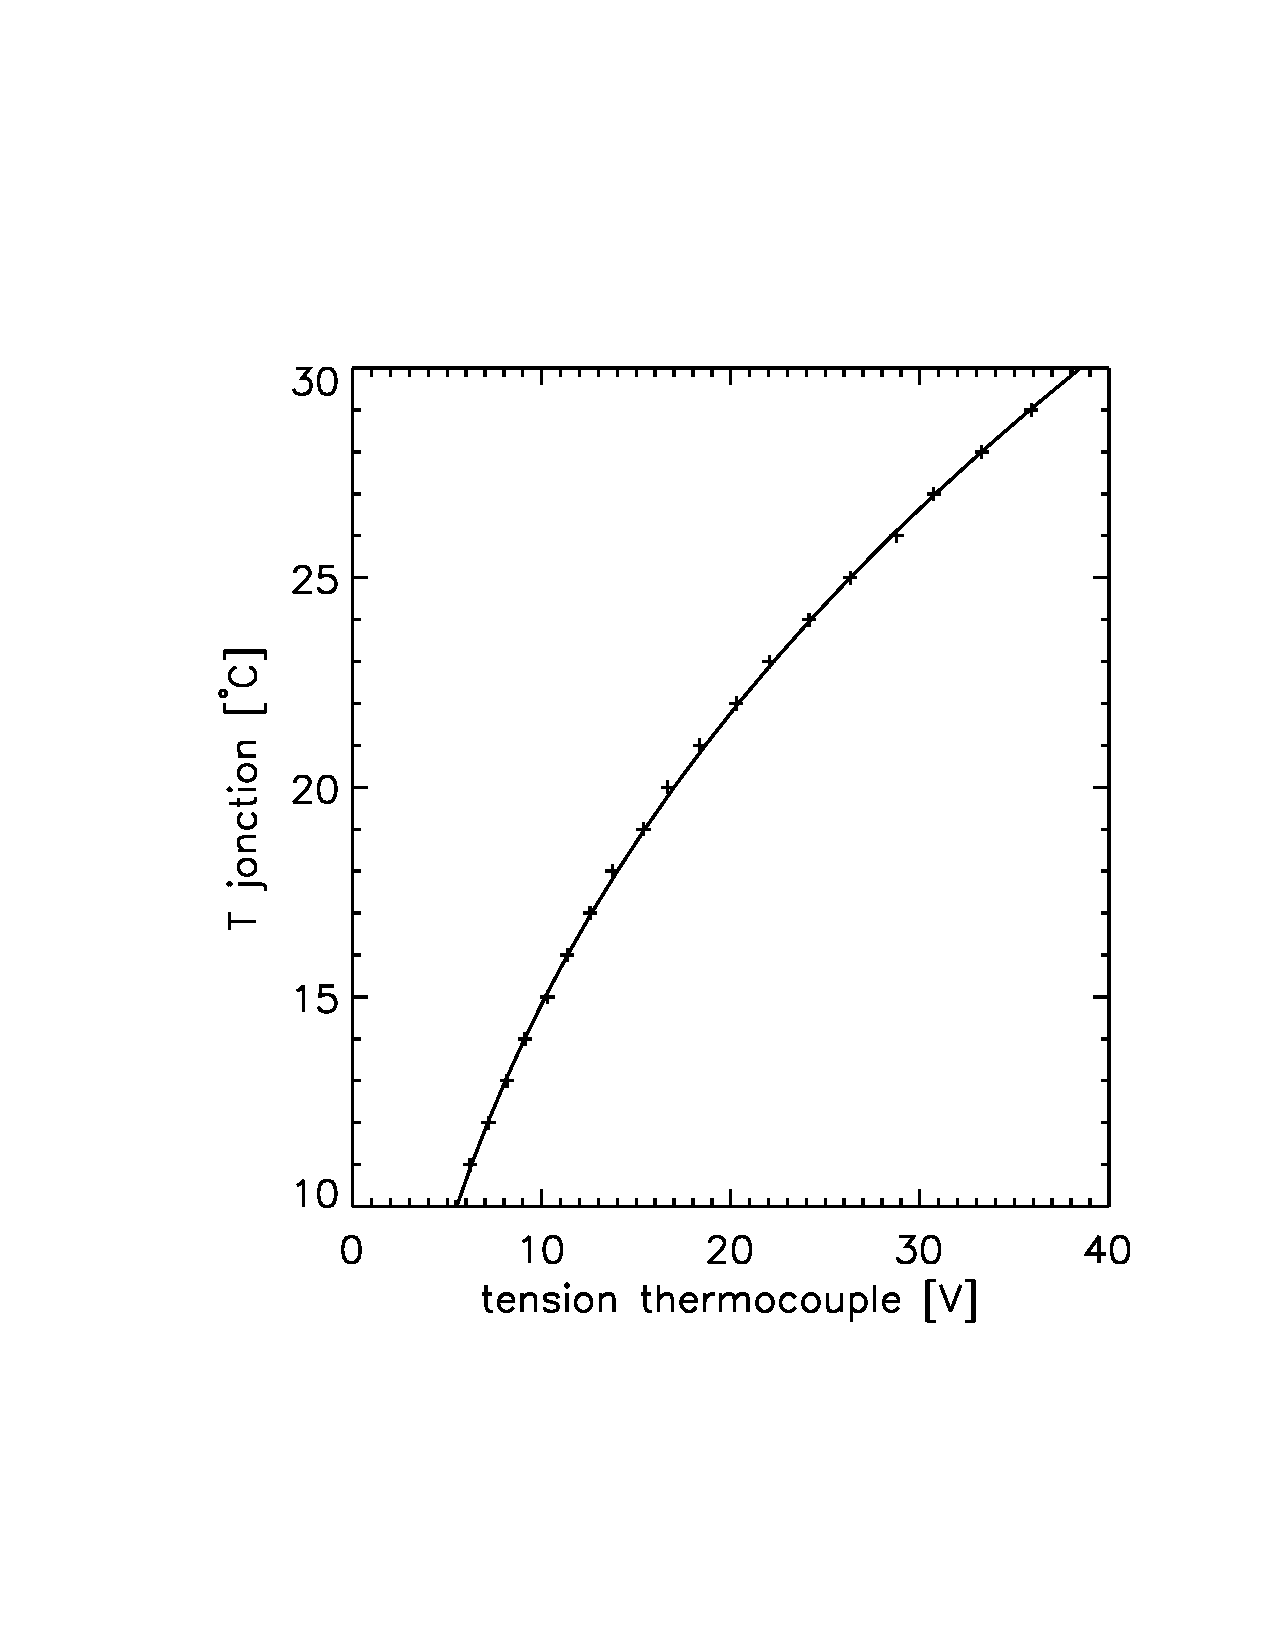
\includegraphics[width=7cm]{assets/figures/calibThermoCouple.pdf}
    \caption{Courbe de calibration du thermocouple (polynôme de degré 4).}
    \label{fig:tc}
\end{wrapfigure}
\paragraph{5/ précision de la calibration.} Bien entendu, puisqu'on effectue un ajustement de modèle - et que tout ajustement est forcément une approximation, car la mesure de calibration est aussi soumise à une erreur - il est important de connaitre la précision à laquelle on doit s'attendre lorsque l'on utilise la courbe de calibration. Ce niveau de sophistication est indispensable pour les mesures à très haute précision (physique fondamentale). Dans l'exemple du thermocouple, on trouve par exemple qu'avec le modèle d'ordre 4, la précision est de 0.054$^\circ$C (table~\ref{tab:tc2}).

\subsection{L'étendue de mesure}\label{sec:etd}

(inspiré de \texttt{wikipedia}). C'est le domaine de variation du mesurande auquel l'instrument est sensible. L'étendue est définie par une valeur minimale: la \textbf{portée minimale}, et une valeur maximale: la \textbf{portée maximale}. Par exemple, un voltmètre pourrait avoir une étendue de mesure de 1 mV à 100 V.

\subsection{La résolution}

(inspiré de \texttt{wikipedia}). La résolution d'un appareil est la plus petite variation du mesurande qui produit une variation perceptible de l'indication délivrée par l'instrument. Elle peut aussi être exprimée en nombre de points de résolution, qui sont alors le nombre de valeurs différentes que l'instrument peut afficher. Par exemple un multimètre de 2000 points pour une étendue de 2 V peut afficher toutes les valeurs comprises entre 0.000 V et 1.999 V; sa résolution est donc de 1 mV.

On rencontre également une autre notation: un appareil sera dit " 3 point 1/2 " au lieu de " 2000 points ". Cela signifie que l'instrument peut afficher une mesure avec trois chiffres après la virgule, plus un " demi chiffre ", un chiffre affiché qui ne peut pas prendre toutes les valeurs (par exemple, le chiffre avant la virgule, qui ne peut prendre que les valeurs 0 ou 1). Dans le cas du multimètre, le " 3 point " est associé aux 3 chiffres après la virgule nécessaire pour exprimer les valeurs de 0.000 V à 1.999 V, et le " 1/2 " est associé aux 0 et 1 avant la virgule.

\subsection{La sensibilité}

La \textbf{sensibilité} (notée $\mathcal{K}$) d'un instrument est définie par la pente de la courbe d'étalonnage $\mathcal{C}(M)$
$$
    \mathcal{K}(M)=\frac{\text{d}\,\mathcal{C}(M)}{\text{d}M}
$$
Elle caractérise l'influence d'un changement de la valeur d'entrée sur la valeur de sortie. Elle n'est constante que si l'instrument est parfaitement linéaire, c.-à-d. si sa courbe d'étalonnage est une droite de pente constante (un changement de la valeur d'entrée $\Delta M$ produit un même changement de la valeur de sortie, quelque soit la valeur de $M$). Dans les autres cas, la sensibilité de l'instrument va varier d'une extrémité à l'autre de son étendue (\ref{sec:etd}). Un bon instrument devra avoir une grande sensibilité.

\subsection{La justesse}

La justesse d'un instrument (notée $\mathcal{J}$) décrit sa capacité à fournir la vraie valeur du mesurande - en imaginant que toutes les sources d'erreur aléatoire ont été éliminées. Il ne reste donc que l'erreur systématique, qui comme on l'a vu plus haut peut être éliminée par étalonnage. On pourrait cependant imaginer des appareils impossibles à calibrer de manière interne (correction automatique impossible) et pour lesquels il soit utile de connaitre la justesse. La correction de calibration serait alors appliquée sur les valeurs données par l'instrument.

L'étalonnage permet de déduire la justesse de l'instrument. En entrant une valeur connue, on peut mesurer l'erreur due à l'instrument et caractériser la justesse par
$$
    \mathcal{J}\ [\%]=100\left(1-\left|\frac{\text{valeur étalon - valeur mesurée}}{\text{valeur étalon}}\right|\right)
$$
Un appareil sans erreur systématique est donc un appareil à 100\% de justesse.

\subsection{La fidélité, ou précision}

Imaginons un instrument à 100\% de justesse. La fidélité ou précision d'une mesure avec un tel instrument indique l'accord typique moyen (en valeur absolue) entre le résultat d'une mesure et la vraie valeur du mesurande. L'écart entre la mesure et la vraie valeur du mesurande est dû aux erreurs aléatoires imprédictibles et non compensables qui se présentent toujours dans les instruments réels (effets thermiques, mécaniques, perturbations électriques, etc.) Un instrument infiniment précis fournirait une mesure exactement égale à la valeur du mesurande.

En d'autres termes, la précision est une mesure de la fluctuation aléatoire des caractéristiques physiques des composants de l'instrument: plus l'instrument est stable, plus il sera précis. Puisque l'erreur interne est de nature aléatoire, la précision se caractérise par l'écart-type moyen entre mesure $M$ et valeur exacte du mesurande (on utilisera un étalon $E$)
$$
    \mathcal{P}=\sqrt{\langle[M-E]^2\rangle}
$$
La précision s'exprime naturellement dans les mêmes unités que le mesurande, et on notera encore que la précision peut tout à fait varier à travers l'étendue de l'instrument.

\subsection{L'exactitude = justesse + précision}

Un instrument de mesure est d'autant plus exact que les résultats de mesure qu'il indique coïncident avec la vraie valeur du mesurande. Il est à remarquer que l'exactitude ne s'exprime pas par une valeur chiffrée. C'est une appréciation qualitative des résultats.

L'exactitude d'un appareil est essentiellement liée à la justesse et la fidélité. \textbf{Un appareil est exact s'il est à la fois juste et précis}. Voir la figure~\ref{fig:exact}.

\begin{figure}[htbp]
    \centering
    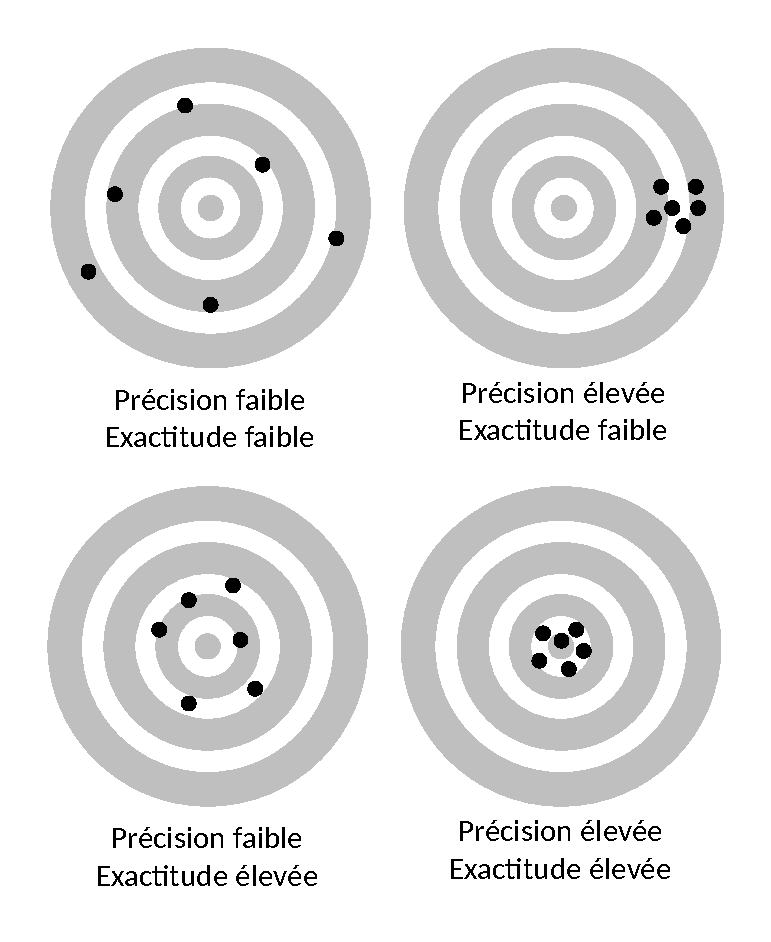
\includegraphics[width=12cm]{assets/figures/juste-fidèle-précis.pdf}
    \caption{On peut représenter symboliquement la fidélité, la justesse et l'exactitude de la manière ci-dessus. Dans le premier cas, les mesures sont proches les unes des autres (bonne fidélité) mais en dehors de la zone de probabilité de la valeur vraie (mauvaise justesse). Dans le deuxième cas, les mesures sont au contraire bien dans la zone oé se trouve la valeur vraie et le " barycentre " des points est au centre de la zone rouge (bonne justesse) mais bien que bonnes, les mesures sont dispersées entre elles (mauvaise fidélité). Enfin, le dernier cas présente des mesures justes (dans la zone de la valeur vraie) et fidèles (proches les unes des autres). C'est le cas d'un bon appareil de mesure, à qui l'apport d'une correction n'est a priori pas nécessaire et les mesures effectuées avec l'appareil sont exactes.}
    \label{fig:exact}
\end{figure}

\subsection{La répétabilité}

Une mesure est qualifiée de \textbf{répétable} lorsqu'il existe un accord entre les résultats des mesures \textbf{successives} du même mesurande (c.-à-d. séparées dans le temps), effectuées dans les \textbf{mêmes} conditions de mesure, c'est-à-dire :
\begin{itemize}
    \item même instrument de mesure,
    \item même procédé de mesure,
    \item même observateur,
    \item même emplacement,
    \item répétition sur une courte période de temps (afin que la relation de calibration reste constante).
\end{itemize}
La dispersion naturelle entre les résultats des mesures individuelles du mesurande dans les conditions ci-dessus, permettra de donner une estimation quantitative de la répétabilité d'une mesure. Le contre-exemple d'une mesure non répétable correspond au cas oé à chaque mesure, le résultat est différent, avec des variations largement supérieures à ce que l'on pourrait s'attendre \underline{compte tenu de la précision de l'instrument}.

\subsection{La reproductibilité}

Une mesure est qualifiée de \textbf{reproductible} lorsqu'il existe un accord entre les résultats des mesures du même mesurande effectuées dans des \textbf{conditions de mesure différentes}. Par exemple, afin d'obtenir un statut universellement accepté par la communauté scientifique, le résultat d'une expérience scientifique destinée au test d'une théorie doit impérativement pouvoir être retrouvé (aux erreurs de mesure près) dans tout laboratoire convenablement équipé. Dans le cas contraire, la théorie testée ne saurait être considérée comme une théorie vraie. Une théorie non vérifiable n'a aucune valeur.

Considérons par exemple le cas de la détermination de la masse du proton, une constante fondamentale en physique nucléaire. Le premier laboratoire ayant réalisé cette mesure a bien entendu publié son résultat dans des revues scientifiques, et d'autres laboratoires à travers le monde se sont empressés de reproduire l'expérience, localement, afin de contrôler l'affirmation du premier laboratoire. Si aucun de ces laboratoires n'avait réussi à reproduire le résultat initial, malgré tous les soins apportés à la mesure et à la minimisation des erreurs, la valeur publiée par le premier laboratoire aurait été rejetée - à raison - par la communauté scientifique. En d'autres termes: \textbf{une mesure non reproductible, ce n'est pas de la science !}\footnote{pour cette simple raison, l'astrologie, la numérologie, l'homéopathie et autres fadaises - ne sauraient accéder au statut de vérité scientifique: \textbf{aucun résultat ni prédiction} de ces machins n'a jamais pu être reproduit ! Jamais ! Seule la naïveté humaine est une certitude universelle.}
